\documentclass[a4paper,14pt,oneside,final]{extarticle}
\usepackage[top=2cm, bottom=2cm, left=3cm, right=1cm]{geometry}
\usepackage{scrextend}

\usepackage[T2A,T1]{fontenc}
\usepackage[ukrainian,russian,english]{babel}
\usepackage{tempora}
\usepackage{fontspec}
\setmainfont{tempora}

% Зачем: Отключает использование изменяемых межсловных пробелов.
% Почему: Так не принято делать в текстах на русском языке.
\frenchspacing

\usepackage{indentfirst}
\setlength{\parindent}{1.25cm}
\renewcommand{\baselinestretch}{1.5}

% Header
\usepackage{fancyhdr}
\pagestyle{fancy}
\fancyhead{}
\fancyfoot{}
\fancyhead[R]{\small \selectfont \thepage}
\renewcommand{\headrulewidth}{0pt}

% Captions
\usepackage{chngcntr}
\counterwithin{figure}{section}
\counterwithin{table}{section}
\usepackage[tableposition=top]{caption}
\usepackage{subcaption}
\DeclareCaptionLabelFormat{gostfigure}{Рисунок #2}
\DeclareCaptionLabelFormat{gosttable}{Таблиця #2}
\DeclareCaptionLabelSeparator{gost}{~---~}
\captionsetup{labelsep=gost}
\captionsetup[figure]{labelformat=gostfigure}
\captionsetup[table]{labelformat=gosttable}
\renewcommand{\thesubfigure}{\asbuk{subfigure}}

% Sections
\usepackage[explicit]{titlesec}
\newcommand{\sectionbreak}{\clearpage}

\titleformat{\section}
  {\centering}{\thesection \quad}{0pt}{\MakeUppercase{#1}}
\titleformat{\subsection}[block]
  {\bfseries}{\thesubsection \quad #1}{0cm}{}

\titlespacing{\section} {0cm}{0cm}{21pt}
\titlespacing{\subsection} {\parindent}{21pt}{0cm}
\titlespacing{\subsubsection} {\parindent}{0cm}{0cm}

% Lists
\usepackage{enumitem}
\renewcommand\labelitemi{--}
\setlist[itemize]{noitemsep, topsep=0pt, wide}
\setlist[enumerate]{noitemsep, topsep=0pt, wide, label=\arabic*}
\setlist[description]{labelsep=0pt, noitemsep, topsep=0pt, leftmargin=2\parindent, labelindent=\parindent, labelwidth=\parindent, font=\normalfont}

% Toc
\usepackage{tocloft}
\tocloftpagestyle{fancy}
\renewcommand{\cfttoctitlefont}{}
\setlength{\cftbeforesecskip}{0pt}
\renewcommand{\cftsecfont}{}
\renewcommand{\cftsecpagefont}{}
\renewcommand{\cftsecleader}{\cftdotfill{\cftdotsep}}

\usepackage{float}
\usepackage{pgfplots}
\usepackage{graphicx}
\usepackage{multirow}
\usepackage{amssymb,amsfonts,amsmath,amsthm}
\usepackage{csquotes}

\usepackage{listings}
\lstset{basicstyle=\footnotesize\ttfamily,breaklines=true}
\lstset{language=Matlab}

\usepackage[
	backend=biber,
	sorting=none,
	language=auto,
	autolang=other
]{biblatex}
\DeclareFieldFormat{labelnumberwidth}{#1}


\newcommand{\labnumber}{2} % second lab
\documentclass[a4paper,14pt,oneside,final]{extarticle}
\usepackage[top=2cm, bottom=2cm, left=3cm, right=1cm]{geometry}
\usepackage{scrextend}

\usepackage[T2A,T1]{fontenc}
\usepackage[ukrainian,russian,english]{babel}
\usepackage{tempora}
\usepackage{fontspec}
\setmainfont{tempora}

% Зачем: Отключает использование изменяемых межсловных пробелов.
% Почему: Так не принято делать в текстах на русском языке.
\frenchspacing

\usepackage{indentfirst}
\setlength{\parindent}{1.25cm}
\renewcommand{\baselinestretch}{1.5}

% Header
\usepackage{fancyhdr}
\pagestyle{fancy}
\fancyhead{}
\fancyfoot{}
\fancyhead[R]{\small \selectfont \thepage}
\renewcommand{\headrulewidth}{0pt}

% Captions
\usepackage{chngcntr}
\counterwithin{figure}{section}
\counterwithin{table}{section}
\usepackage[tableposition=top]{caption}
\usepackage{subcaption}
\DeclareCaptionLabelFormat{gostfigure}{Рисунок #2}
\DeclareCaptionLabelFormat{gosttable}{Таблиця #2}
\DeclareCaptionLabelSeparator{gost}{~---~}
\captionsetup{labelsep=gost}
\captionsetup[figure]{labelformat=gostfigure}
\captionsetup[table]{labelformat=gosttable}
\renewcommand{\thesubfigure}{\asbuk{subfigure}}

% Sections
\usepackage[explicit]{titlesec}
\newcommand{\sectionbreak}{\clearpage}

\titleformat{\section}
  {\centering}{\thesection \quad}{0pt}{\MakeUppercase{#1}}
\titleformat{\subsection}[block]
  {\bfseries}{\thesubsection \quad #1}{0cm}{}

\titlespacing{\section} {0cm}{0cm}{21pt}
\titlespacing{\subsection} {\parindent}{21pt}{0cm}
\titlespacing{\subsubsection} {\parindent}{0cm}{0cm}

% Lists
\usepackage{enumitem}
\renewcommand\labelitemi{--}
\setlist[itemize]{noitemsep, topsep=0pt, wide}
\setlist[enumerate]{noitemsep, topsep=0pt, wide, label=\arabic*}
\setlist[description]{labelsep=0pt, noitemsep, topsep=0pt, leftmargin=2\parindent, labelindent=\parindent, labelwidth=\parindent, font=\normalfont}

% Toc
\usepackage{tocloft}
\tocloftpagestyle{fancy}
\renewcommand{\cfttoctitlefont}{}
\setlength{\cftbeforesecskip}{0pt}
\renewcommand{\cftsecfont}{}
\renewcommand{\cftsecpagefont}{}
\renewcommand{\cftsecleader}{\cftdotfill{\cftdotsep}}

\newcommand{\khpistudentgroup}{КН-34г}
\newcommand{\khpistudentname}{Чепурний~А.~С.}

\newcommand{\khpidepartment}{Програмна інженерія та інформаційні технології управління}
\newcommand{\khpititlewhat}{
	Лабораторна робота №\labnumber \\
	з предмету <<Моделювання систем>>
}
\newcommand{\khpititlewho}{
	Виконав: \\
	\hspace*{\parindent} ст. групи \khpistudentgroup \\
	\hspace*{\parindent} \khpistudentname \\
	Перевірила: \\
	\hspace*{\parindent} ст. в. каф. ПІІТУ \\
	\hspace*{\parindent} Єршова~С.~І. \\
	\hspace*{\parindent} ас. каф. ПІІТУ \\
	\hspace*{\parindent} Литвинова~Ю.~С. \\
}



\graphicspath{{figures/}}

\begin{document}
\Ukrainian

\begin{titlepage}

\begin{center}
	МІНІСТЕРСТВО ОСВІТИ І НАУКИ УКРАЇНИ \\
	НАЦІОНАЛЬНИЙ ТЕХНІЧНИЙ УНІВЕРСИТЕТ \\
	«ХАРКІВСЬКИЙ ПОЛІТЕХНІЧНИЙ ІНСТИТУТ» \\[0.5cm]
	Кафедра <<\khpidepartment>> \\
\end{center}

\vspace{6cm}

\begin{center}
	\khpititlewhat
\end{center}

\vspace{3cm}

\begin{addmargin}[10cm]{0cm}
	\khpititlewho
\end{addmargin}

\vspace{\fill}

\begin{center}
	Харків \the\year
\end{center}

\end{titlepage}

\addtocounter{page}{1}

\section*{Розробка вимог щодо програмного забезпечення для моделювання неперервних детермінованих систем}
\subsubsection*{Мета роботи}
Дослідити особливості моделювання неперервних детермінованих систем та отримати практичні навички моделювання програмних вимог.
\subsubsection*{Хід роботи}
\begin{enumerate}
\item Отримати та дослідити неперервний детермінований процес за індивідуальним завданням.
\item Проаналізувати модель, визначити цілі моделювання.
\item Розробити вимоги до програмного забезпечення.
\item Задокументувати розроблені вимоги, використовуючи UML (за допомогою Requirement diagram).
\item Оформити звіт, який повинен містити опис досліджуваного процесу, його модель (диференційні рівняння та їх вирішення), цілі моделювання, опис програмних вимог та моделі програмних вимог, розроблені за допомогою UML.
\end{enumerate}

\subsection{Індивідуальне завдання}
Вантаж з масою $P$ підвішений на вертикальній пружині, довжина якої дорівнює $l$. 
Вантаж злегка відтягнутий донизу і потім відпущений.
Знайти закон руху вантажу, нехтуючи масою пружини та опором повітря.

\subsection{Аналіз та дослідження моделі}
Направимо вісь $O_x$ вниз по вертикальній прямій, що проходить через точку підвісу вантажу.
Початок координат $O$ виберемо в положенні рівноваги вантажу, тобто в точці, в якій вага вантажу врівноважується силою натягу пружини~(рисунок~\ref{fig:problem}).

\begin{figure}[H]
  \centering
    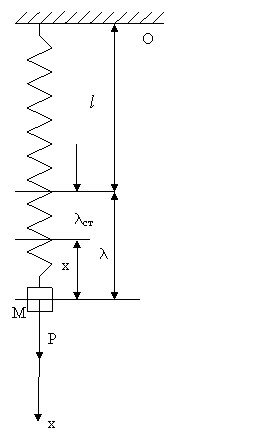
\includegraphics[width=0.4\textwidth]{problem}
  \caption{Деформація розтягу пружини}
  \label{fig:problem}
\end{figure}

Нехай $\lambda$ означає подовження пружини в даний момент, а $\lambda_{st}$ --- статичне подовження, тобто відстань від кінця нерозтягнутої пружини до положення рівноваги. 
Тоді 
\[
\lambda-\lambda_{st}=x
\].

Згідно до закону Гука сила натягу пружини пропорційно її подовженню:
\begin{align*}
F_\textup{пр}&=-kx, \\
P = F_\textup{тяг}&=ma,
\end{align*}
\begin{description}
\item[де] $k$ --- жорсткість пружини.
\end{description}

При цьому виконується наступне співвідношення:
\begin{align*}
F_\textup{тяг} &= F_\textup{пр}, \\
ma &= -kx.
\end{align*}

Останній вираз приведемо до нормального вигляду однорідного диференціального рівняння другого порядку, що описує одновимірний (з одним ступенем свободи) рух пружинного маятника:
\[
m\cfrac{d^2x}{dt^2} + \omega^2x = 0,
\]
\begin{description}
\item[де] $\omega^2 = \cfrac{k}{m}$.
\end{description}

Отримане рівняння визначає так звані вільні коливання вантажу.
Воно називається рівнянням гармонічного осцилятора.
Це лінійне диференціальне рівняння другого порядку з постійними коефіцієнтами.
Його загальне рішення:
\[
x = C_1 \cos \omega t + C_2 \sin \omega t.
\]

Для з'ясування фізичного сенсу рішення зручніше привести його до іншої форми, помноживши та поділивши на $\sqrt{C_1^2 + C_2^2}$:
\[
x = \sqrt{C_1^2 + C_2^2} \cdot \left( \cfrac{C_1}{\sqrt{C_1^2 + C_2^2}} \cos \omega t + \cfrac{C_2}{\sqrt{C_1^2 + C_2^2}} \sin \omega t \right).
\]

Якщо покласти, що
\begin{align*}
\sqrt{C_1^2 + C_2^2} &= A, \\
\cfrac{C_1}{\sqrt{C_1^2 + C_2^2}} &= \sin \phi, \\
\cfrac{C_2}{\sqrt{C_1^2 + C_2^2}} &= \cos \phi,
\end{align*}

тоді
\begin{align*}
x &= A \cdot (\sin\phi \cdot \cos \omega t + \cos\phi \cdot \sin \omega t) = \\
&= A \cdot \sin (\omega t + \phi) = \\
&= A \cdot \sin (\sqrt{\frac{k}{m}} \cdot t + \phi),
\end{align*}
\begin{description}
\item[де] $A$ --- амплітуда коливання;
\item $\omega$ --- циклічна частота коливань пружинного маятника.
\end{description}

Швидкість руху вантажу виходить диференціюванням рішення:
\[
v=\cfrac{dx}{dt}=A\cdot\cos(\omega t+\phi).
\]

\subsection{Вимоги до програмного забезпечення}
\subsubsection{Функціональні вимоги}
Список функціональних вимог системи представлено у UML-нотації на рисунку~\ref{fig:usecase}.

\begin{figure}[H]
  \centering
    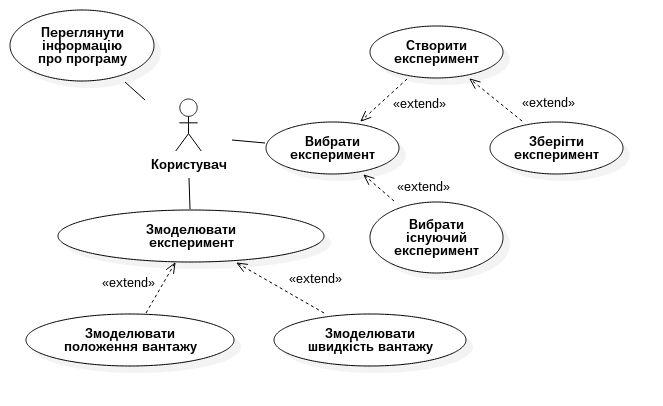
\includegraphics[width=1\textwidth]{uml_usecase}
  \caption{Діаграма варіантів використання}
  \label{fig:usecase}
\end{figure}

\subsubsection{Нефункціональні вимоги}
Список нефункціональних вимог системи:
\begin{enumerate}[label={\arabic*)}]
	\item зручний інтерфейс;
	\item сучасний стиль графічного інтерфейсу;
	\item використання бази даних SQLite.
\end{enumerate}

\subsection{Функціональна модель}
Функціональну модель процесу моделювання представлено у IDEF-нотації на рисунках~\ref{fig:idef0_l1} та~\ref{fig:idef0_l2}.

\begin{figure}[H]
  \centering
    
\includegraphics[width=0.5\textwidth]{idef0_l1}
  \caption{Діаграма IDEF0 моделювання (концептуальний рівень)}
  \label{fig:idef0_l1}
\end{figure}

\begin{figure}[H]
  \centering
    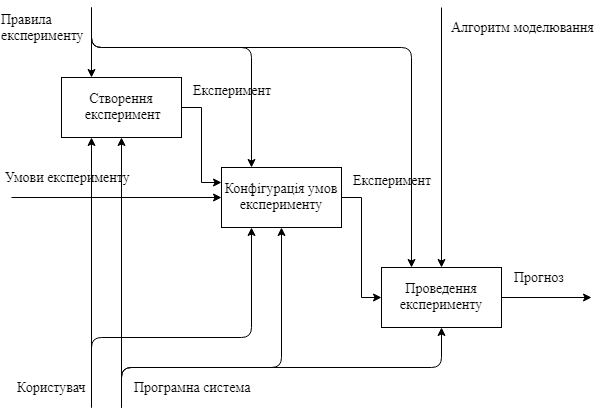
\includegraphics[width=.9\textwidth]{idef0_l2}
  \caption{Діаграма IDEF0 моделювання}
  \label{fig:idef0_l2}
\end{figure}

\end{document}
